\documentclass[ignorenonframetext,]{beamer}
\setbeamertemplate{caption}[numbered]
\setbeamertemplate{caption label separator}{:}
\setbeamercolor{caption name}{fg=normal text.fg}
\usepackage{amssymb,amsmath}
\usepackage{ifxetex,ifluatex}
\usepackage{fixltx2e} % provides \textsubscript
\usepackage{lmodern}
\ifxetex
  \usepackage{fontspec,xltxtra,xunicode}
  \defaultfontfeatures{Mapping=tex-text,Scale=MatchLowercase}
  \newcommand{\euro}{€}
\else
  \ifluatex
    \usepackage{fontspec}
    \defaultfontfeatures{Mapping=tex-text,Scale=MatchLowercase}
    \newcommand{\euro}{€}
  \else
    \usepackage[T1]{fontenc}
    \usepackage[utf8]{inputenc}
      \fi
\fi
% use upquote if available, for straight quotes in verbatim environments
\IfFileExists{upquote.sty}{\usepackage{upquote}}{}
% use microtype if available
\IfFileExists{microtype.sty}{\usepackage{microtype}}{}
\usepackage{graphicx}
\makeatletter
\def\maxwidth{\ifdim\Gin@nat@width>\linewidth\linewidth\else\Gin@nat@width\fi}
\def\maxheight{\ifdim\Gin@nat@height>\textheight0.8\textheight\else\Gin@nat@height\fi}
\makeatother
% Scale images if necessary, so that they will not overflow the page
% margins by default, and it is still possible to overwrite the defaults
% using explicit options in \includegraphics[width, height, ...]{}
\setkeys{Gin}{width=\maxwidth,height=\maxheight,keepaspectratio}



\setlength{\parindent}{0pt}
\setlength{\parskip}{6pt plus 2pt minus 1pt}
\setlength{\emergencystretch}{3em}  % prevent overfull lines
\setcounter{secnumdepth}{0}

\usepackage{amsmath,verbatim}

\usepackage{fancyvrb}
\usepackage{manfnt}
\usepackage[normalem]{ulem}

%\usepackage[colorlinks=true]{hyperref}

\mode<presentation>{\usetheme{Malmoe}}

%\synctex=1

\setbeamertemplate{headline}{}


\setbeamerfont{footline}{size=\scriptsize}
\setbeamerfont{frametitle}{shape=\scshape}
\setbeamertemplate{itemize items}[circle]
\setbeamercovered{transparent}

\setbeamertemplate{navigation symbols}{}
\setbeamertemplate{footline}[frame number]{} 


\definecolor{forest}{rgb}{0, .5, 0}
\definecolor{brick}{rgb}{.5, 0, 0}
\definecolor{darkgreen}{rgb}{0, .5, 0}
\definecolor{darkred}{rgb}{.7, .15, .15}
\definecolor{darkblue}{rgb}{0, 0, .5}
\definecolor{Green}{rgb}{0.2,1,0.2}


\newcommand{\R}{\textsf{R}}
\newcommand{\RStudio}{\textsl{R Studio}}


\usepackage[english]{babel}
%\usepackage{palatino}
\usepackage[T1]{fontenc}


% make all tt fonts bold to look more like Verbatim
\usepackage{lmodern}
\renewcommand\ttfamily{\usefont{T1}{lmtt}{m}{n}}

% Comment these out if you don't want a slide with just the
% part/section/subsection/subsubsection title:
\AtBeginPart{
  \let\insertpartnumber\relax
  \let\partname\relax
  \frame{\partpage}
}
\AtBeginSection{
  \let\insertsectionnumber\relax
 \let\sectionname\relax
 \frame{\sectionpage}
}
\AtBeginSubsection{
  \let\insertsubsectionnumber\relax
  \let\subsectionname\relax
  \frame{\subsectionpage}
}

\title{Models for fev}
\author{NEJM Course for Medical Reporters}
\date{September 12 \& 19, 2016}

\begin{document}
\frame{\titlepage}

\begin{frame}
\tableofcontents[hideallsubsections]
\end{frame}

\begin{frame}[fragile]{Unadjusted association}

\begin{verbatim}
## 
## Call:
## lm(formula = fev$fev ~ smoking.status)
## 
## Coefficients:
##       (Intercept)  smoking.statusYes  
##             2.566              0.711
\end{verbatim}

\end{frame}

\begin{frame}[fragile]{A model based adjustment}

\begin{verbatim}
## 
## Call:
## lm(formula = fev$fev ~ smoking.status + fev$Age)
## 
## Coefficients:
##       (Intercept)  smoking.statusYes            fev$Age  
##             0.367             -0.209              0.231
\end{verbatim}

\end{frame}

\begin{frame}[fragile]{Another model based adjustment}

\begin{verbatim}
## 
## Call:
## lm(formula = fev$fev ~ smoking.status + fev$Age + fev$Sex + fev$Hgt)
## 
## Coefficients:
##       (Intercept)  smoking.statusYes            fev$Age  
##           -4.4570            -0.0872             0.0655  
##           fev$Sex            fev$Hgt  
##            0.1571             0.1042
\end{verbatim}

\end{frame}

\begin{frame}[fragile]{Another model}

\begin{verbatim}
## 
## Call:
## lm(formula = fev$fev ~ smoking.status + fev$Age + fev$Hgt)
## 
## Coefficients:
##       (Intercept)  smoking.statusYes            fev$Age  
##           -4.6160            -0.1102             0.0597  
##           fev$Hgt  
##            0.1091
\end{verbatim}

\end{frame}

\begin{frame}{Stratification}

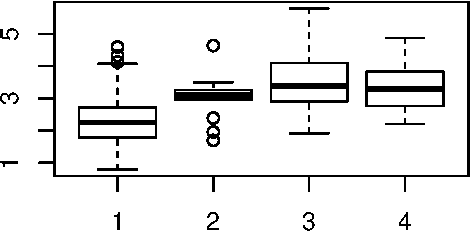
\includegraphics{fev_models_files/figure-beamer/unnamed-chunk-5-1.pdf}\\

\end{frame}

\end{document}
